\MySection{Introduction}
\MySubSection{extended Higgs sector}
\Slide{t}{
Many BSM theories need to enlarge their Higgs sector to two Higgs doublets
\begin{itemize}%1
  % https://arxiv.org/pdf/1706.07414.pdf (page 11)
\item The minimal \acp{2HDM} predict 5 physical states:
  \begin{itemize}%2
    \item two neutral, \CP-even particles \Ph\ and \PH\ ( $\mh \leq \mH$)
    \item one neutral, \CP-odd particle \PSAz
    \item two charged Higgs bosons \PHpm
  \end{itemize}%2
\end{itemize}%1

\vspace{0.35cm}

\acs{SM} fermion coupling to 2HDs (no \acsp{FCNC}):
\twoColumnsAsymAlt
    {
      \small
      \begin{itemize}
      \item[\alertA{I}] \alertA{All quarks \& leptons couple to $\Phi_{2}$}
        \vspace{-0.08cm}
      \item[\alertB{II}] \alertB{All $u$-type to $\Phi_{2}$ and all $d$-type \& $\ell$ to $\Phi_{1}$} %\NeutralTag{MSSM-like}
        \vspace{-0.08cm}
      \item[\alertC{X}] \alertC{Both $u$ \& $d$ types couple to $\Phi_{2}$, all $\ell$ to $\Phi_{1}$}
        \vspace{-0.08cm}
      \item[\alertD{Y}] \alertD{Roles of two doublets reversed wrt \Type{II}}
      \end{itemize}
    }
    {
      \vspace{-0.25cm}
      
      \resizebox{0.87\linewidth}{!}{
        % https://arxiv.org/pdf/1607.01320.pdf
%\note{The most popular models of the Yukawa interactions in the 2HDM 
%  (also referred to as ``Types''). The symbols $u$, $d$, $\ell$ refer to up-
%  and down-type quarks, and charged leptons of any generation.
%  Here, $\Phi_1$ and $\Phi_2$ refer to the Higgs doublet coupled to
%  the particular fermion.}
\resizebox{0.65\linewidth}{!}{
  \begin{tabular}{l c c c}
    \hline
    Type & $u$ & $d$ & $\ell$ \\
    \hline
    \rowcolor{\ColourA}
    I & $\Phi_2$ & $\Phi_2$ & $\Phi_2$
    \\%[0.1cm]
    \rowcolor{\ColourB}
    II & $\Phi_2$ & $\Phi_1$ & $\Phi_1$ %\NeutralTag{MSSM}\\
    \\
    \rowcolor{\ColourC}
    III (X) & $\Phi_2$ & $\Phi_2$ & $\Phi_1$
    \\%[0.1cm]
    \rowcolor{\ColourD}
    IV (Y)  & $\Phi_2$ & $\Phi_1$ & $\Phi_2$
    \\%[0.1cm]
    \hline
  \end{tabular}}


      }
    }

\vspace{0.45cm}
    
For each \acsp{2HDM} type there are 7 free parameters (incl. \mh, \mH, \mA, \mHpm):
\begin{enumerate}
  \setcounter{enumi}{4}
\item \tanbetaDef, the ratio of the Higgs doublet \acsp{VEV}
\item \sinba, \mixingAngle: the mixing angle of the \CP-even states
\item \massMatrixDiagonal, diagonal term of the mass matrix of the Higgs doublets

\end{enumerate}
}

\MySubSection{production $\&$ decay}
\Slide{t}{
Three mass categories are commonly defined in \PHpm\ searches:
\begin{itemize}
\item \alertA{Light $\mHpm < \mtop - \mbottom$ },
  \alertB{intermediate\tikzmark{f0} $\mHpm \sim \mtop$},
  \alertC{heavy $\mHpm > \mtop + \mbottom$}
\end{itemize}

\vspace{0.2cm}               
Decay \acsp{BR} model-dependent $\Rightarrow$ different searches constrain different scenarios.

% https://arxiv.org/pdf/2005.08900.pdf
\twoFigColumns
{LHCHXSWG_v1/LowTanBetaM50to200/mh125_brs_tanb0p5}{$M_{h}^{125}$,
  \tanbeta = 0.5}
{LHCHXSWG_v1/LowTanBetaM90to1000/mh125_br_tb}{ $M_{h}^{125}$, \PHpm $\rightarrow$ tb}
{0.8}

\vspace{0.2cm}

\textbf{\acsp{BR} of \textcolor{kGreen}{\PHpm $\rightarrow$ tb}
  dominanates at high $\mHpm$, for wide range of \tanbeta}
}

\MySubSection{final state}
\Slide{t}{

  \vspace{0.1cm}
  
This analysis searches for a heavy \PHpm

\vspace{-0.1cm}

\threeFigColumnsCustomSize
    {paper/feynman/hplus_4FS}{4FS}
    {paper/feynman/hplus_5FS}{5FS}
    {paper/feynman/hplus_sChannel}{s-channel}
    {0.85}

    \vspace{0.5cm}
    
    \textbf{\textcolor{kBlue}{Fully-hadronic} final state of associated production characterised by}:

  \twoColumns
      {

        \vspace{0.25cm}
        
        \begin{itemize}
          \small
        \item High jet \& \bjet\ multiplicities 
        \item[\Good] Large branching ratio $\BR\simeq46\%$
        %\item Absence of neutrinos $\Rightarrow$ low \ptmiss
        \item[\Good] Invariant mass reconstruction of \PHpm
        \item[\Bad] QCD multijet \& \ttbar background % irreducible
        \item[\Bad] Combinatorial (self-)background
        \end{itemize}
      }
      {        
        \vspace{-0.25cm}
        {\oneFig{tikz/pdf/HPlus4FS_HToTB_FH}{0.9}}
      }
}

\MySubSection{topology}
\Slide{t}{
       Various $\mathrm{m_{H^\pm}}$ reconstruction techniques
       available due to signal process kinematics:

       \vspace{0.1cm}       

    \begin{itemize}
      \small
    \item\textcolor{kDarkGreen}{\textbf{Resolved \PQt}:} At moderate
      \mHpm\ \& \ptHpm the decay products of \PHpm are well separated
    \item \textcolor{kBlue}{\textbf{Boosted \PW/\PQt\tikzmark{bW1}}:}
      As $\mathrm{m_{H^\pm}}$ increases the \PHpm\ decay products
      become boosted
    \item \textcolor{kOrange}{\textbf{Boosted \Hpm}:} As \ptHpm
      increases its decay products become collinear \tikzmark{bH1}      
    %\item As the $\mathrm{p_{T,H^{\pm}}}$ increases, its decay
      %products become collinear
    \end{itemize}

    \vspace{0.1cm}
    
  \begin{columns}[T]
      \begin{column}{0.20\textwidth}
        \begin{tcolorbox}[transparentStyle, title=\tColorBoxTitle{\tikzmark{rTop2}\vspace{-0.15cm}\resolvedTop}]
          \oneFig{tikz/pdf/h2tb_ResolvedTop}{1.0}
        \end{tcolorbox}
      \end{column}
      \begin{column}{0.20\textwidth}
        \begin{tcolorbox}[transparentStyle, title=\tColorBoxTitle{\tikzmark{bW2}\vspace{-0.15cm}\boostedW}]
        \oneFig{tikz/pdf/h2tb_BoostedW}{1.0}
        \end{tcolorbox}
      \end{column}
      \begin{column}{0.20\textwidth}
        \begin{tcolorbox}[transparentStyle,  opacitytext=1.0, title=\tColorBoxTitle{\tikzmark{bTop}\vspace{-0.15cm}\boostedTop}]
        \oneFig{tikz/pdf/h2tb_BoostedTop}{1.0}
        \end{tcolorbox}
      \end{column}
       \begin{column}{0.20\textwidth}
         \begin{tcolorbox}[transparentStyle, title=\tColorBoxTitle{boosted \PHpm}\vspace{-0.15cm}\tikzmark{bH2}]
         \oneFig{tikz/pdf/h2tb_Boostedhiggs}{1.0}
          \end{tcolorbox}
      \end{column}
      \begin{column}{0.20\textwidth}
        \begin{tcolorbox}[transparentStyle, title=\tikzmark{bH3}\tColorBoxTitle{\vspace{-0.15cm}boosted \PHpm}]
          \oneFig{tikz/pdf/h2tb_BoostedhiggsLargePt}{1.0} 
        \end{tcolorbox}
      \end{column}
  \end{columns}

  \vspace{0.35cm}
  
  \twoColumns
      {
        \small
        \hspace{1.5cm} \textbf{Previous results}
        \vspace{0.1cm}
        \CustomiseLineSpacing{0.95}
        \begin{itemize}
        \item \textcolor{kDarkGreen}{\textbf{Resolved \PQt}},
          \textcolor{kBlue}{\textbf{Boosted \PW/\PQt}}\newline studied separately by dedicated analyses
        \item 2016 ReReco data
        \item CADI \href{https://cms.cern.ch/iCMS/analysisadmin/cadilines?line=HIG-18-015}{\textcolor{kBlue}{HIG-18-015}}
        \end{itemize}
      }
      {
        \small
        \hspace{2cm}  \textbf{This work}
        \vspace{0.1cm}
        \CustomiseLineSpacing{0.95}
        \begin{itemize}          
          \item \textcolor{kDarkGreen}{\textbf{Resolved \PQt}},
            \textcolor{kBlue}{\textbf{Boosted \PQt}},  \textcolor{kBlue}{\textbf{Boosted W}}
          \item Full Run II data
          \item This talk: status of 2018 data
            %\item Last progress report in HExtended meeting:
          \item Last report (HExtended):
            \href{https://indico.cern.ch/event/1071752/contributions/4578521/attachments/2333742/3977531/HiggsExtended_MKolosova_25Oct2021.pdf}{\textcolor{kBlue}{25
            Oct 2021}}
        \end{itemize}        
      }
}

\MySection{Previous results}
\MySubSection{review}
\Slide{t}{

  
  \hspace{4.0cm} \textcolor{kDarkGreen}{\textbf{Resolved}}   \RectangleText{\href{https://cms.cern.ch/iCMS/analysisadmin/cadilines?line=HIG-18-015}{\Large CADI: HIG-18-015}}%(UCY, HIP)

  \vspace{0.1cm}

  %\CustomiseLineSpacing{1.1}  
  \begin{itemize}
    \small
  \item Resolved t ($t^{res}$) identification: custom top tagger (BDT)
  \item Selected events contain $\ge$ 7 jets, $\ge$ 3 b-tagged, 2 $t^{res}$
  \item \PHpm mass reconstruction ($m_{bt}$): leading \pT $t^{res}$ +
    leading \pT b jet
  \item Main background:
    \begin{itemize}
      \footnotesize
    \item Misid. B: From data using CRs (ABCD method)
    \item Genuine B: from simulation
    \end{itemize}
  \item $m_{bt}$ is used to extract the signal in the presence of the SM background.
  \end{itemize}

  \vspace{-0.2cm}
  
  \twoFigColumns
      {CMS-HIG-18-015/Figure_003-a.pdf}{$t^{res}$ efficiency}
      %{topEffic_Resolved_HIG18015}{$t^{res}$ efficiency}
      {CMS-HIG-18-015/Figure_005-b.pdf}{$m_{bt}$ Post-fit}
      {0.55}
}

\Slide{t}{

  \hspace{4.0cm} \textcolor{kBlue}{\textbf{Boosted}}   \RectangleText{\href{https://cms.cern.ch/iCMS/analysisadmin/cadilines?line=HIG-18-015}{\Large CADI: HIG-18-015}}%(MIT, BUAP)  

  \vspace{0.05cm}  

  \begin{itemize}
    \small
  \item Events are split in four main categories
  \end{itemize}

  \vspace{-0.4cm}
  
  \begin{columns}[T]
      \begin{column}{0.145\textwidth}
        \begin{tcolorbox}[transparentStyle,
            title=\tColorBoxTitle{\vspace{-0.15cm} t0b}]
          \oneFig{tikz/pdf/h2tb_HIG-18-015_t0b_2bjets}{1.0}
        \end{tcolorbox}
      \end{column}
      \begin{column}{0.145\textwidth}
        \begin{tcolorbox}[transparentStyle,
            title=\tColorBoxTitle{\vspace{-0.15cm} t1b}]
        \oneFig{tikz/pdf/h2tb_HIG-18-015_t1b_2bjets}{1.0}
        \end{tcolorbox}
      \end{column}
      \begin{column}{0.145\textwidth}
        \begin{tcolorbox}[transparentStyle,  opacitytext=1.0,
            title=\tColorBoxTitle{\vspace{-0.15cm} Wbb}]
        \oneFig{tikz/pdf/h2tb_HIG-18-015_Wbb_2bjets}{1.0}
        \end{tcolorbox}
      \end{column}
       \begin{column}{0.145\textwidth}
         \begin{tcolorbox}[transparentStyle,
             title=\tColorBoxTitle{\vspace{-0.15cm} Wbj}]
         \oneFig{tikz/pdf/h2tb_HIG-18-015_Wbj_1bjets.pdf}{1.0}
          \end{tcolorbox}
      \end{column}
  \end{columns}

  \vspace{-0.2cm}
  %\oneFigColumns{boosted_categories.png}{}{0.85}

  \begin{itemize}
    \small
  \item Boosted $t$/$W$ identification: Based on \mSD[],
    \subjettiness[]{N}, $N_{b \ \text{subjets}}$
  \item \PHpm mass reconstruction ($m_{bt}$): $t$ + leading \pT b jet
  \item Further categorization according to:
    \begin{itemize}
      \setlength{\itemindent}{1mm}
      \footnotesize
    \item $N_{b}$ $\in [=1, =2, \geq 3]$
    \item $N_{j}^{extra}$ $\in [< 3, \geq 3]$
    \item \mHpmReco $\in [\text{below}, \text{in}, \text{above}]$ of FWHM of signal
    %\item Number of bjets (=1, =2, $\ge$3)
    %\item Number of jets not used in \PHpm (<3, $\ge$ 3)
    %\item Below, in and above the $m_{bt}$ window
    \end{itemize}
  \end{itemize}

  %\vspace{-0.1cm}

  \twoColumns
      {
        \begin{itemize}
          \small
        \item Main background
          \begin{itemize}
            \footnotesize
          \item[QCD]: from data using CRs (inverted
            \subjettiness[]{N}), sidebands with \mHpmReco
            $\in [\text{below},\text{above}]$)
          \item[\ttbar]: from sim., normalized in CR with 1
            $\ell$
          \end{itemize}
        \end{itemize}
      }
      {
        
        \vspace{-2.7cm}
        \oneFigColumns{CMS-HIG-18-015/Figure_005-a.pdf}{}{0.57}
      }

      \vspace{-0.1cm}
      
      \begin{itemize}
        \small
        \item $H_{T}$ is used to extract the signal from SM background inside the $m_{bt}$ window.
      \end{itemize}
}

\Slide{t}{

  Upper limits on $\sigma_{\mathrm{H}^{\pm}t(b)}\times\mathcal{B}(\mathrm{H}^{\pm} \to \mathrm{tb})$

  \vspace{-0.5cm}
  
  \twoFigColumns
      {limit_assoc_HIG18015}{}
      {CMS-HIG-18-015/Boosted_Figure-aux_001-b.pdf}{}
      {0.9}

  \vspace{0.4cm}
      
  \twoColumns
      {
        \begin{itemize}
          \footnotesize
        \item Resolved and Boosted overlayed limits
        \item No excess above the estimated background
        \item Interpretation in hMSSM:
          max. \tanb = 0.88 excluded for \mHpm~=~0.20-0.55~TeV
        \end{itemize}
      }
      {        
        \begin{itemize}
          \footnotesize
        \item Boosted analysis categories
        \item Most sensitive category is $t1b$
        \item Least sensitive category is $Wbj$
        \end{itemize}
      }
}

\MySection{This work}
\MySubSection{strategy}
\Slide{t}{

  \textbf{Three main categories with different topology}

  \begin{enumerate}
    \small
  \item 2 resolved tops
  \item 1 resolved $\&$ 1 boosted top
  \item 2 boosted tops
  \end{enumerate}

  \vspace{0.3cm}

  \begin{itemize}
    \small
  \item This analysis targets full Run II data
  \item This talk presents a study using 2018 data (RunIISummer20UL18)
  \end{itemize}

  \begin{center}
    \resizebox{0.7\linewidth}{!}{%https://tex.stackexchange.com/questions/38177/including-large-tables-in-a-beamer-frame
      \begin{tabular}{ll}
        \textbf{Datasets}
        & \multicolumn{1}{c}{\textbf{Luminosity ($\mathrm{pb^{-1}}$)}} \\ \hline
        JetHT\_Run2018A\_UL2018\_MiniAODv2\_v1\_315257\_316995 & 14026.95\\ 
        JetHT\_Run2018B\_UL2018\_MiniAODv2\_v1\_317080\_319310 & 7060.79\\ 
        JetHT\_Run2018C\_UL2018\_MiniAODv2\_v1\_319337\_320065 & 6894.78\\ 
        JetHT\_Run2018D\_UL2018\_MiniAODv2\_v2\_320413\_325172 & 31834.89\\
        \hline
        \multicolumn{1}{r}{Total:}                                                 & 59817.41
    \end{tabular}}
  \end{center}

  \vspace{0.15cm}

  \begin{itemize}
    \small
  \item MC simulated samples include:
  \end{itemize}
  \twoColumnsAsymAlt
      {
        \begin{itemize}          
          \vspace{-0.35cm}
        \item[ ]
          \begin{itemize}
            \footnotesize
          \item Signal: $\mHpm = 200 - 3000$ GeV (17 points)
          \item QCD (\HT binned)
          \item Top (Single top, \ttbar, \ttbar+X)
          \item V+jets, diboson, triboson
          \end{itemize}
      \end{itemize}
      }
      {

      }
}

%\MySection{Resolved}
\MySection{ }
\begin{frame}[noframenumbering]{}
  \begin{center}
    \huge \textbf{Resolved analysis}
  \end{center}
\end{frame}

\MySection{Strategy}

\Slide{t}{

  \textbf{Signal region (SR):}
  \vspace{+0.2cm}
  \begin{center}
    \resizebox{0.8\linewidth}{!}{
      \begin{tabular}{l l}
        \hline
        \cellcolor[gray]{.9}Trigger  & \cellcolor[gray]{.9}$H_{T}$ + multijet + 1 or 2 b jets\\
        $\ell(\tau_{h})$ veto & \pT > 10(20) GeV, $|\eta|$ < 2.4(2.3)\\
        %$e$ veto & \pT > 10 GeV, $|\eta|$ < 2.4, Loose miniIso, cutBasedElectronID (veto) \\%\_Fall17\_94X\_V2\_veto \\
        %\cellcolor[gray]{.9}$\mu$ veto & \cellcolor[gray]{.9}\pT > 10 GeV, $|\eta|$ < 2.4, Loose miniIso isCutBasedIDLoose\\
        %$\tau$ veto & \pT > 20 GeV, $|\eta|$ < 2.3, DeepTau \dDeepTau[vloose]{\Pe}, \dDeepTau[medium]{\mu}, \dDeepTau[loose]{j}\\
        \cellcolor[gray]{.9}$\ge$ 7 jets & \cellcolor[gray]{.9}$p_{T}^{6th}$ > 40 GeV, $p_{T}^{7th}$ > 30 GeV, $|\eta|$ < 2.4, Tight ID\\
        $H_{T}$ > 500 GeV & \\
        \cellcolor[gray]{.9}$\ge$ 3 b jets & \cellcolor[gray]{.9}\pT > 40 GeV, DeepJet Medium WP \\
        $\ge$ 2 resolved top ($t^{res}$)
        &  \begin{tabular}{@{}l@{}}$130 < m_{\mathrm{t^{res}}} <
             210~$GeV\\ medium (loose) WP: 5(10)$\%$ misID rate\end{tabular}\\
        \hline
      \end{tabular}
    }
  \end{center}

  \vspace{0.75cm}
  
  
  \twoColumnsAsymAlt
      {
        \normalsize
        $\ \ $ \textbf{SR categorization based on $t^{res}$}
        \begin{itemize}
          \small
        \item \textcolor{kDarkGreen}{$1M1L_{t^{res}}$}: medium
          $t^{res}_{p_{T,1}}$ \newline
          \textcolor{white}{$1M1L_{t^{res}}$:} loose-not-medium
          $t^{res}_{p_{T,2}}$
        \item \textcolor{kDarkGreen}{$2M_{t^{res}}$}: both $t^{res}$ medium tagged
        \end{itemize}

        \vspace{0.3cm}

        $\ \ $ \textbf{Invariant \PHpm~mass reconstruction}:
        \begin{itemize}
          \large
        \item[] \textcolor{kOrange}{\mHpmReco = $t^{res}_{p_{T,1}}$
          + b$_{p_{T,1}}$}
        \end{itemize}
      }
      {
        \vspace{-0.4cm}
        \oneFigColumns{tikz/pdf/HPlus4FS_HToTB_ResolvedTop_InvMass}{}{1.0}%\mHpmReco=\rTop$_{ \ ldg \ p_{T}}$ + bjet$^{free}_{ldg \ p_{T}}$}{0.68}
      }
}

\MySection{Top tagging}
\Slide{t}{
  \small

  \vspace{0.1cm}

  A fully connected NN is developed to reconstruct resolved top-quarks

  \begin{itemize}
  \item Distinguishes trijets from top-quark decays and trijets from combinatorial background.
  \end{itemize}

  \vspace{-0.1cm}
  
  \begin{columns}[T]
    \begin{column}{0.014\textwidth}
    \end{column}
     \begin{column}{0.52\textwidth}
       \small    
       \begin{itemize}
       \item Training on simulated $t\bar{t}$ events
         \begin{itemize}
           \small
         \item \textcolor{kDarkGreen}{Signal:} truth-matched trijets
         \item \textcolor{kRed}{Background:} non-matched trijets
         \item[] \footnotesize{\textcolor{white}{Background:} ($\ge$ 1 non-matched jet)}
        \end{itemize}
       \end{itemize}
     \end{column}
     \begin{column}{0.47\textwidth}
       %\vspace{-0.2cm}
       \twoFigColumns
           {top-training/top_matched}{ \textcolor{kDarkGreen}{signal}}
           {top-training/top_unmatched1b}{\textcolor{kRed}{background}}
           {0.5}
     \end{column}
     \begin{column}{0.01\textwidth}\end{column}
  \end{columns}

  \vspace{-0.05cm}
  
  Mass decorrelation using sample reweighting:

  \begin{itemize}
    \small
  %\item Input variables are uncorrelated to the top-quark mass distribution ($m_{top}$)
  \item \textcolor{kRed}{Background} is reweighted such that $m_{top}$ matches the \textcolor{kDarkGreen}{signal}.
  \end{itemize}

  \vspace{-0.3cm}

  \threeColumns
      {\oneFigColumns{CMS-HIG-21-010_Figure_003.pdf}{}{1.0}}
      {\oneFigColumns{topTagging/trijetMass_3WPs}{}{1.0}}
      {
          
        \footnotesize
        \vspace{1.3cm}

        Calibration performed

        \vspace{0.5cm}
        
        %\begin{itemize}
        %  \scriptsize
        %\item[] In \href{http://cms-results.web.cern.ch/cms-results/public-results/publications/HIG-21-010/index.html}{\textcolor{kBlue}{HIG-21-010}}
        %\item[] Documentation: \href{https://cms.cern.ch/iCMS/user/noteinfo?cmsnoteid=CMS\%20AN-2021/019}{\textcolor{kBlue}{AN 2021/019}}
        %\item[] Approved by \href{https://indico.cern.ch/event/1042288/contributions/4380251/attachments/2256031/3920589/updated_TopTag_JMAR_06Jul2021.pdf}{\textcolor{kBlue}{JMAR group}}
        %\end{itemize}
        \href{http://cms-results.web.cern.ch/cms-results/public-results/publications/HIG-21-010/index.html}{\textcolor{kBlue}{HIG-21-010}}
        Submitted to JHEP\newline
        \vspace{0.1cm}Documentation: \href{https://cms.cern.ch/iCMS/user/noteinfo?cmsnoteid=CMS\%20AN-2021/019}{\textcolor{kBlue}{AN 2021/019}}\newline
        \vspace{0.1cm}Approved by \href{https://indico.cern.ch/event/1042288/contributions/4380251/attachments/2256031/3920589/updated_TopTag_JMAR_06Jul2021.pdf}{\textcolor{kBlue}{JMAR group}}

      }

      %\PlaceText{73mm}{65mm}{\scriptsize{\textcolor{kBlue}{loose}}}
      %\PlaceText{67mm}{72mm}{\tiny{\textbf{Loose WP}}}
      \PlaceText{67mm}{65mm}{\boxed{\tiny{\textbf{Loose WP}}}}
}
  
\MySection{Background}
\Slide{t}{

  \vspace{0.1cm}
  
  %\small
  Main background for the \PHpm $\rightarrow$ tb fully hadronic final
  state:

  \vspace{0.1cm}
  
  \begin{itemize}
    \small
  \item QCD multijet \DataDrivenTag
  \item EWK processes (mainly \ttbar) \SimulationTag
  \end{itemize}

  \vspace{0.35cm}

  \normalsize
  \textbf{QCD background measurement}\newline
  \small
  %\textbf{Defining 3 orthogonal control regions (CR) for each SR}:\newline
  %\textbf{Use discriminating variables to define 3 orthogonal control regions (CR) for each SR}:

  \vspace{-0.25cm}
  
  Defining 3 orthogonal control regions (CR) for each SR

  \vspace{-0.2cm}
  \twoColumnsAsymAlt
      {
        \begin{itemize}
        \small
        \item \textcolor{kRed}{$t^{res}_{assoc}$ mass}: On-mass
          $\rightarrow$ Off-mass ``sidebands''
        \item \textcolor{kRed}{$t^{res}_{H^{\pm}}$ mva}: t-tagged (t) $\rightarrow$ non t-tagged (!t)
        \end{itemize}
      }
      {
      }

  \vspace{0.45cm}
      
  ``ABCD'' method
  
  \twoColumnsAsymAlt
      {
        \begin{equation*}
          \boxed{\textcolor{black}{N^{SR}_{QCD}} =
            \sum_{i}^{\mathrm{bins}} \textcolor{black}{N^{CR(off\texttt{-}m,t)}_{QCD,i}}  \cdot \left(\frac{\textcolor{black}{N^{CR(on\texttt{-}m,!t)}_{QCD,i}}}{\textcolor{black}{N^{CR(off\texttt{-}m,!t)}_{QCD,i}}} \right)}
        \end{equation*}
        
        \vspace{-0.1cm}
        \begin{itemize}
          \footnotesize
        \item Performed in bins of the $t^{res}_{assoc}$ \pT:
          \begin{itemize}
            \footnotesize
          \item $2M_{t^{res}}$: \pT $\in$ [0, 100, 300, $\infty$] GeV
          \item $1M1L_{t^{res}}$: \pT $\in$ [0, 175, $\infty$] GeV 
          \end{itemize}          
        \end{itemize}        
      }
      {

        \vspace{-1.6cm}
        
        \oneFigColumns{qcdSidebands.pdf}{Sidebands}{1.0}
      }
}

\MySubSection{Validation}
\Slide{t}{

  \normalsize
  \textbf{Two validation regions (VRs) for each SR}

  \begin{itemize}    
    \footnotesize
  \item \ttbar enriched: $ \ \ \ \ ==$ 2 b jets, $m_{t^{res}_{H^{\pm}}} \in$ [145, 195] GeV, $\Delta R_{min}(bb)$ > 1.2
  \item  QCD enriched: $==$ 2 b jets, $m_{t^{res}_{H^{\pm}}} \notin$ [145, 195] GeV, $\Delta R_{min}(bb)$ < 0.9
  \end{itemize}

  \begin{columns}[T]
    \begin{column}{0.01\textwidth}
    \end{column}
    \begin{column}{0.099\textwidth}

      \vspace{1.25cm}
      \tikz{\overlaynode<indianred,{oxfordblue,rotate=3}>at(0,5)[draw]{$1M1L_{t^{res}}$};}

      \vspace{2.75cm}
      \tikz{\hspace{0.3cm}\overlaynode<indianred,{oxfordblue,rotate=3}>at(0,5)[draw]{$2M_{t^{res}}$};}

    \end{column}
    \begin{column}{0.9\textwidth}

      \vspace{-0.1cm}
      
      \threeFigColumnsCustomSize
          {QCDDataDriven_SR_1T_TopMass50to260_PtBins175_15Nov2022/DataDrivenPlots/TFsFromSR/HPlusMass.pdf}{SR}
          {QCDDataDriven_VRQCD_1T_TopMass50to230_PtBins175_15Nov2022/DataDrivenPlots/TFsFromSR/HPlusMass.pdf}{$VR_{QCD}$}
          {QCDDataDriven_VRTT_1T_TopMass50to260_PtBins175_15Nov2022/DataDrivenPlots/TFsFromSR/HPlusMass.pdf}{$VR_{\ttbar}$}
          {0.76}

          \vspace{-0.55cm}
          
      \threeFigColumnsCustomSize      
          {QCDDataDriven_SR_2T_TopMass50to260_PtBins100to300_17Nov2022/DataDrivenPlots/TFsFromSR/HPlusMass.pdf}{}
          {QCDDataDriven_VRQCD_2T_TopMass50to260_PtBins100to300_15Nov2022/DataDrivenPlots/TFsFromSR/HPlusMass.pdf}{}
          {QCDDataDriven_VRTT_2T_TopMass50to260_PtBins100to300_15Nov2022/DataDrivenPlots/TFsFromSR/HPlusMass.pdf}{}
          {0.76}
    \end{column}
  \end{columns}

      %\PlaceText{17mm}{65mm}{\boxed{\tiny{\textbf{Loose WP}}}}
}

\MySection{Signal extraction}
\Slide{t}{

  A parameterized DNN is developed to extract signal from SM background
  \begin{itemize}
    \small
  \item \textcolor{blue}{Signal}: $H^{\pm} \rightarrow$ tb for different mass hypotheses
  \item \textcolor{red}{Background}: \ttbar $\rightarrow$ SR,
    Combinatorial $\rightarrow$ CR$^{(off\texttt{-}m,t)}$ \TTMCTag
    %\begin{itemize}
    %  \footnotesize
    %\item \ttbar from SR
    %\item Combinatorial from CR$^{(off\texttt{-}m,t)}$ %\textcolor{kGreen}{0 matched-$t_{res}$}
    %\end{itemize}
  %\item Training (test) is done using \ttbar MC of 2017 (2018) data era \OrthogonalityTag
  \end{itemize}

  \twoColumnsAsymOp
  {
    \small
    %\begin{tcolorbox}[colback=white]
    \center{\textbf{\textcolor{oxfordblue}{Input variables}}}
    \vspace{0.1cm}

    \begin{tcolorbox}[colback=white]
    \begin{itemize}
      \CustomiseLineSpacing{0.75}
      \scriptsize
    \item[1] $\Delta \theta$($t_{H+}, b_{H+}$) in $H^{\pm}$ CM
    \item[2] $H_{T,3b}$% = pt($b_{t^{res}_{assoc}}$) + pt($b_{t^{res}_{H^{\pm}}}$) + pt($b_{H^{\pm}}$)
    \item[3] $p_{T}$(bb$_{dRmin}$)
    \item[4] m(bb$_{maxPt}$)
    \item[5] y23 = $p^{2}_{T,j3}/(p_{T,j1}+p_{T,j2})^{2}$%$\frac{p^{2}_{T,j3}}{(p_{T,j1}+p_{T,j2})^{2}}$
    \item[6] $p_{T,b({\PHpm})}$/$H_{T,3b}$%$\frac{p_{T,b_{H+}}}{HTb}$
    \item[7] $m_{H^{\pm}}$
    \item[8] $p_{T}^{Asym}$(\PHpm, b$_{\PHpm}$)
    %\item[8] $\frac{|p_{T,H+} - p_{T,b_{H+}}|}{p_{T,H+} + p_{T,b_{H+}}}$
    \item[9] Circularity
    \item[10] Sphericity
    \item[11] Aplanarity
    \item[12] Number of medium tops
    \item[13] \textcolor{red}{True mass}
      \vspace{-0.15cm}
    \item[]
  \end{itemize}
    \end{tcolorbox}
  }
  {
    \vspace{0.05cm}
    
    \oneFigColumns{parameterizedDNN.png}{\textbf{Parameterized DNN}}{1.0}

    \vspace{0.3cm}

    \begin{itemize}
      \footnotesize
    \item \textcolor{red}{True mass} is the \textcolor{red}{$\theta$} parameter
    \item In background events, the true mass is randomly assigned to the same values used for signal
    \item Training (test) is done using 2017 (2018) data %\OrthogonalityTag
    \end{itemize}
  }    
}

\MySubSection{Parameterized DNN}
\Slide{t}{

  \small
  %ROC curve for various mass hypotheses
  Parameterized DNN is trained using 6 different mass hypotheses.

  \begin{itemize}
    \small
  \item Training masses = [220, 350, 600, 1000, 1500, 2500] GeV \SolidLineTag
  \item Performance compared to DNNs with fixed \mHpm \DashedLineTag
  \end{itemize}

  \twoColumns
      {\oneFigColumns{ROC}{ROC}{1.0}}
      {

	\vspace{1.3cm}

        \begin{itemize}
          \small
        \item Each curve is evaluated at the \newline true mass
          DNN(\textbf{x},\mHpm)
        \item Comparable results!
        \item Good prediction even for masses not given in the training
        \end{itemize}        
      }      
}

\MySection{Signal region}
\Slide{t}{

  \begin{columns}[T]
    \begin{column}{0.01\textwidth}
    \end{column}
    \begin{column}{0.099\textwidth}

      \vspace{1.5cm}
      \tikz{\overlaynode<indianred,{oxfordblue,rotate=3}>at(0,5)[draw]{$1M1L_{t^{res}}$};}

      \vspace{3.5cm}
      \tikz{\hspace{0.3cm}\overlaynode<indianred,{oxfordblue,rotate=3}>at(0,5)[draw]{$2M_{t^{res}}$};}

    \end{column}
    \begin{column}{0.9\textwidth}

      \vspace{-0.1cm}
        
  \threeFigColumnsCustomSize
      {datacards_HToTB_UL2018_13TeV_HToTB_EraRun2018UL_Search350to3000_OptNominal_FakeBFromDataDriven_m200to3000_3B1T_Created20221110_112420/controlPlots/DataDrivenCtrlPlot_M300_MVAOutput_M300_AfterSelections.pdf}{DNN($m_{H^{\pm}}$ = 300 GeV)}
      {datacards_HToTB_UL2018_13TeV_HToTB_EraRun2018UL_Search350to3000_OptNominal_FakeBFromDataDriven_m200to3000_3B1T_Created20221110_112420/controlPlots/DataDrivenCtrlPlot_M600_MVAOutput_M600_AfterSelections.pdf}{DNN($m_{H^{\pm}}$ = 600 GeV)}
      {datacards_HToTB_UL2018_13TeV_HToTB_EraRun2018UL_Search350to3000_OptNominal_FakeBFromDataDriven_m200to3000_3B1T_Created20221110_112420/controlPlots/DataDrivenCtrlPlot_M1250_MVAOutput_M1250_AfterSelections.pdf}{DNN($m_{H^{\pm}}$ = 1250 GeV)}
      {0.9}

      \vspace{-0.3cm}
      
      \threeFigColumnsCustomSize
      {datacards_HToTB_UL2018_13TeV_HToTB_EraRun2018UL_Search350to3000_OptNominal_FakeBFromDataDriven_m200to3000_3B2T_Created20221110_112420/controlPlots/DataDrivenCtrlPlot_M220_MVAOutput_M220_AfterSelections.pdf}{}
      {datacards_HToTB_UL2018_13TeV_HToTB_EraRun2018UL_Search350to3000_OptNominal_FakeBFromDataDriven_m200to3000_3B2T_Created20221110_112420/controlPlots/DataDrivenCtrlPlot_M600_MVAOutput_M600_AfterSelections.pdf}{}
      {datacards_HToTB_UL2018_13TeV_HToTB_EraRun2018UL_Search350to3000_OptNominal_FakeBFromDataDriven_m200to3000_3B2T_Created20221110_112420/controlPlots/DataDrivenCtrlPlot_M1250_MVAOutput_M1250_AfterSelections.pdf}{}
      {0.9}

    \end{column}
  \end{columns}
      
  }

%%%%
\MySubSection{Limits}
\Slide{t}{

  Expected limits on $\sigma_{\mathrm{H}^{\pm}t(b)}\times\mathcal{B}(\mathrm{H}^{\pm} \to \mathrm{tb})$
 
  \threeFigColumnsCustomSize
      {limitsBr_logY_1T.pdf}{$\mathrm{1M1L_{t}}$}
      {limitsBr_logY_2T.pdf}{$\mathrm{2M_{t}}$}
      {limitsBr_logY.pdf}{Combined}
      {1.0}

      \vspace{0.5cm}
      
      \begin{itemize}
        \small
      \item Statistical uncertainties only
      \item Sensitivity comes to a plateau for $m_{H^{\pm}}$ > 1000 GeV
      \item Results improved by a factor of 2 wrt 2016 data analysis \FixmeTag
      \end{itemize}
}

\MySection{ }
\begin{frame}[noframenumbering]{}
  \begin{center}
    \huge \textbf{Boosted analysis}
  \end{center}
\end{frame}

\MySection{Strategy}

\Slide{t}{

  \begin{columns}[T]
    \begin{column}{0.014\textwidth}
    \end{column}
    \begin{column}{0.52\textwidth}
      \small
      \textcolor{white}{xx} \textbf{Two SRs based on the number of} \newline 
      \textcolor{white}{xx} \textbf{boosted tops ($t^{bst}$):}
      \begin{itemize}
        \small
      \item[]% \textbf{Two SRs based on the number of boosted tops ($t^{bst}$):}    
        \vspace{0.2cm}
        \begin{itemize}
          \footnotesize
        \item[\textbf{SR1}]: N$_{t^{bst}}$ == 1
        \item[\textbf{SR2}]: N$_{t^{bst}}$ == 2
        \end{itemize}
      \end{itemize}
    \end{column}
    \begin{column}{0.41\textwidth}      

    \twoFigColumns
        {boostedSR1}{SR1}
        {boostedSR2}{SR2}
        {0.9}
    \end{column}
    \begin{column}{0.07\textwidth}\end{column}
  \end{columns}
      
  \vspace{-0.15cm}

  \tikz{\scriptsize \hspace{4.5cm} \overlaynode<indianred,{oxfordblue,rotate=3}>at(0,3)[draw]{ Preliminary};}
  \begin{center}
    \resizebox{0.87\linewidth}{!}{
      \begin{tabular}{l l l}
        %$\ \ \ \ $ \textbf{\textcolor{oxfordblue}{SR1}} &
        %$\ \ \ \ $ \textbf{\textcolor{oxfordblue}{SR2}} & \\
        %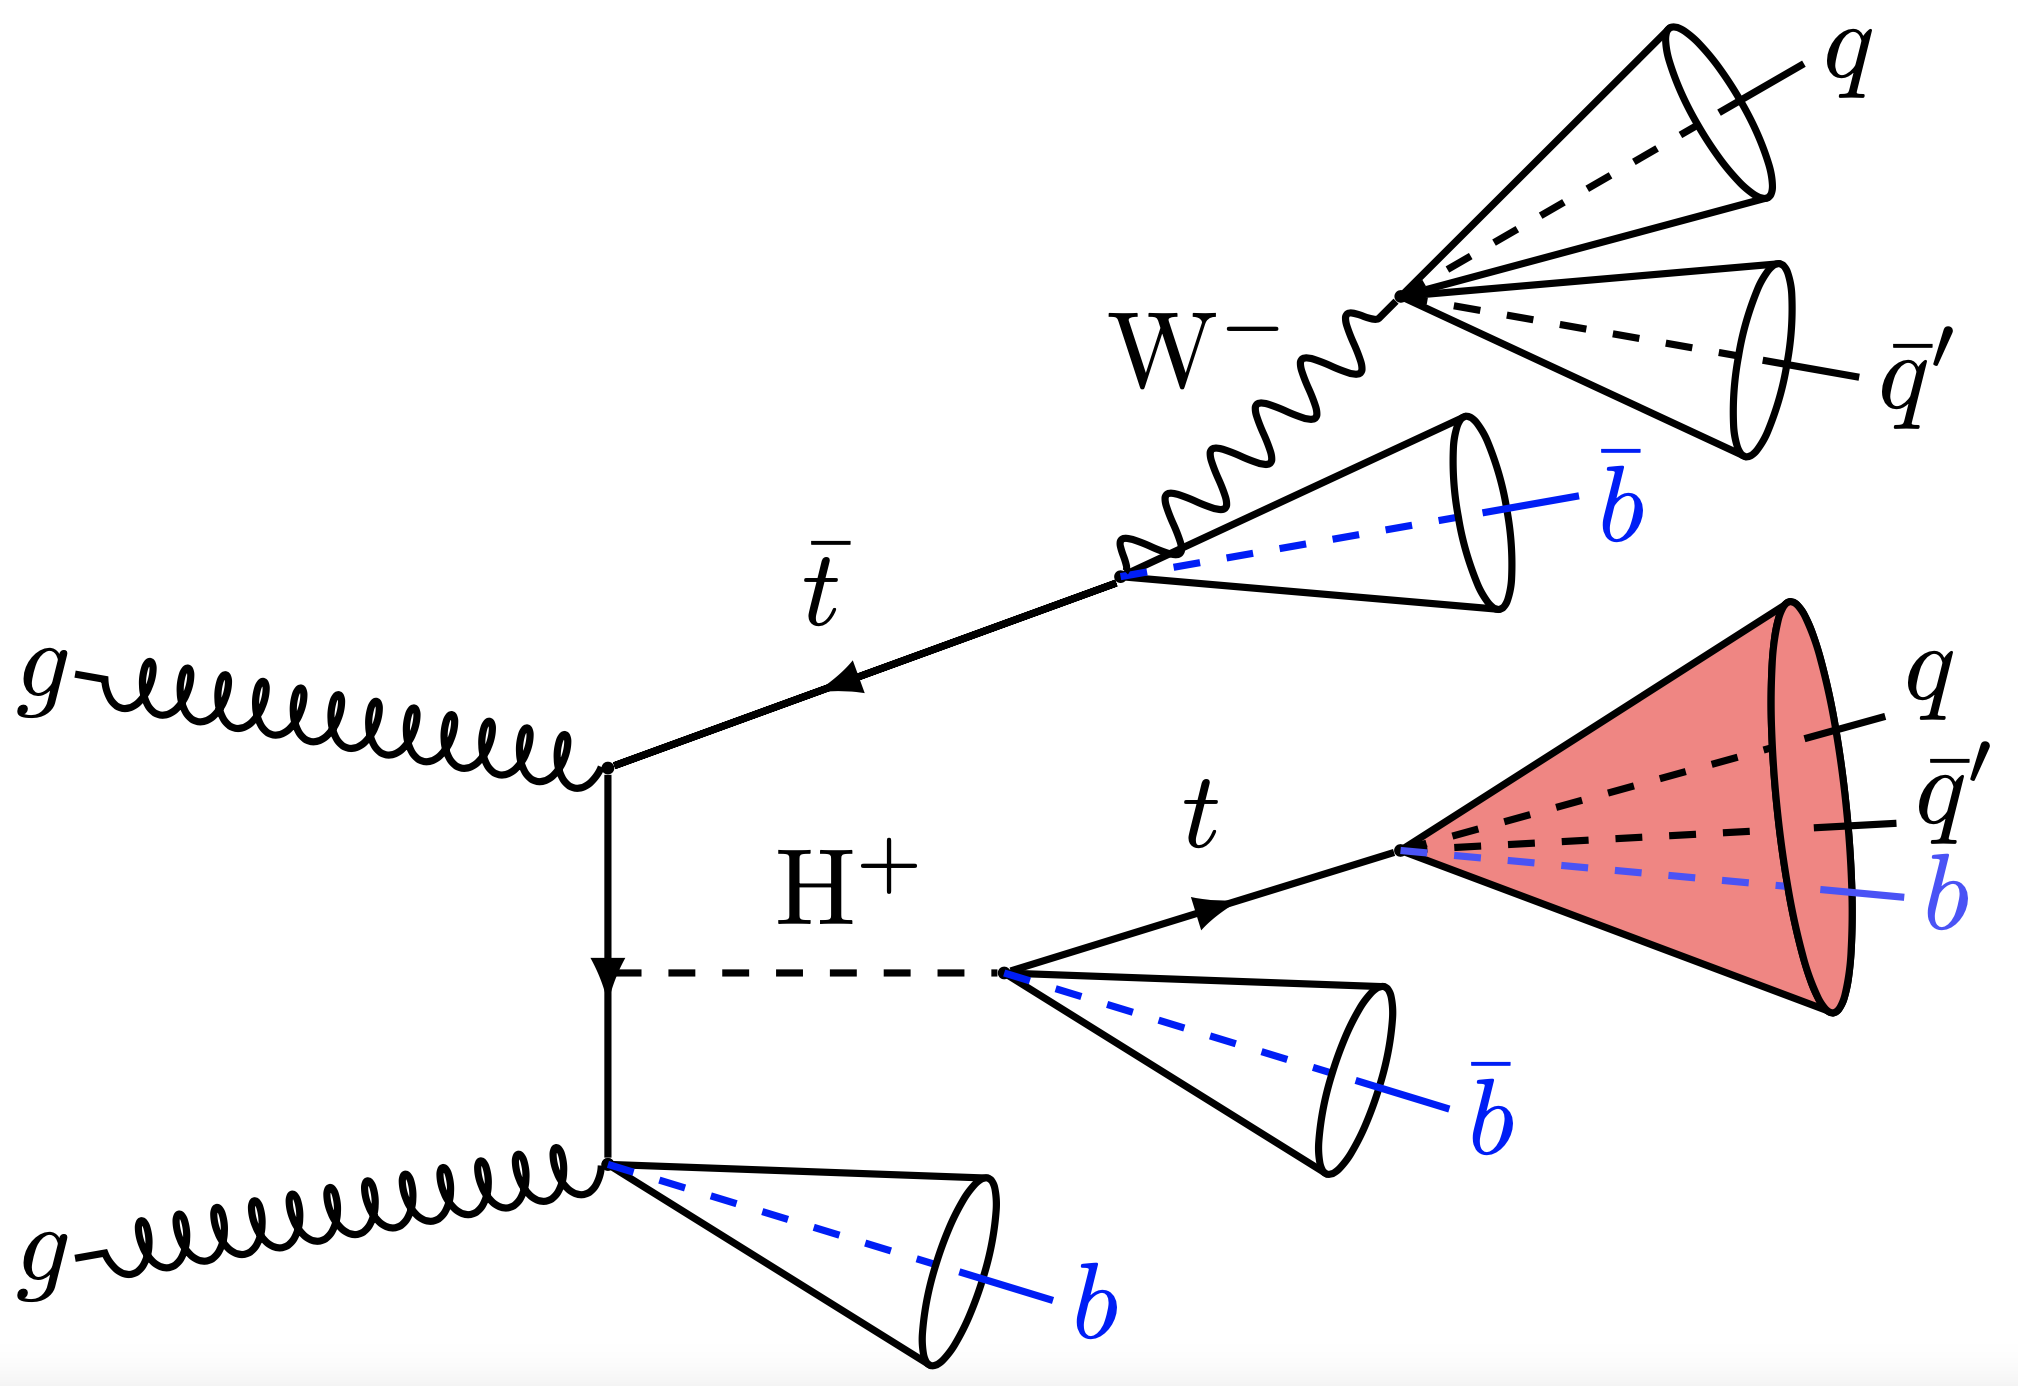
\includegraphics[width=0.2\textwidth]{./figures/boostedSR1} &
        %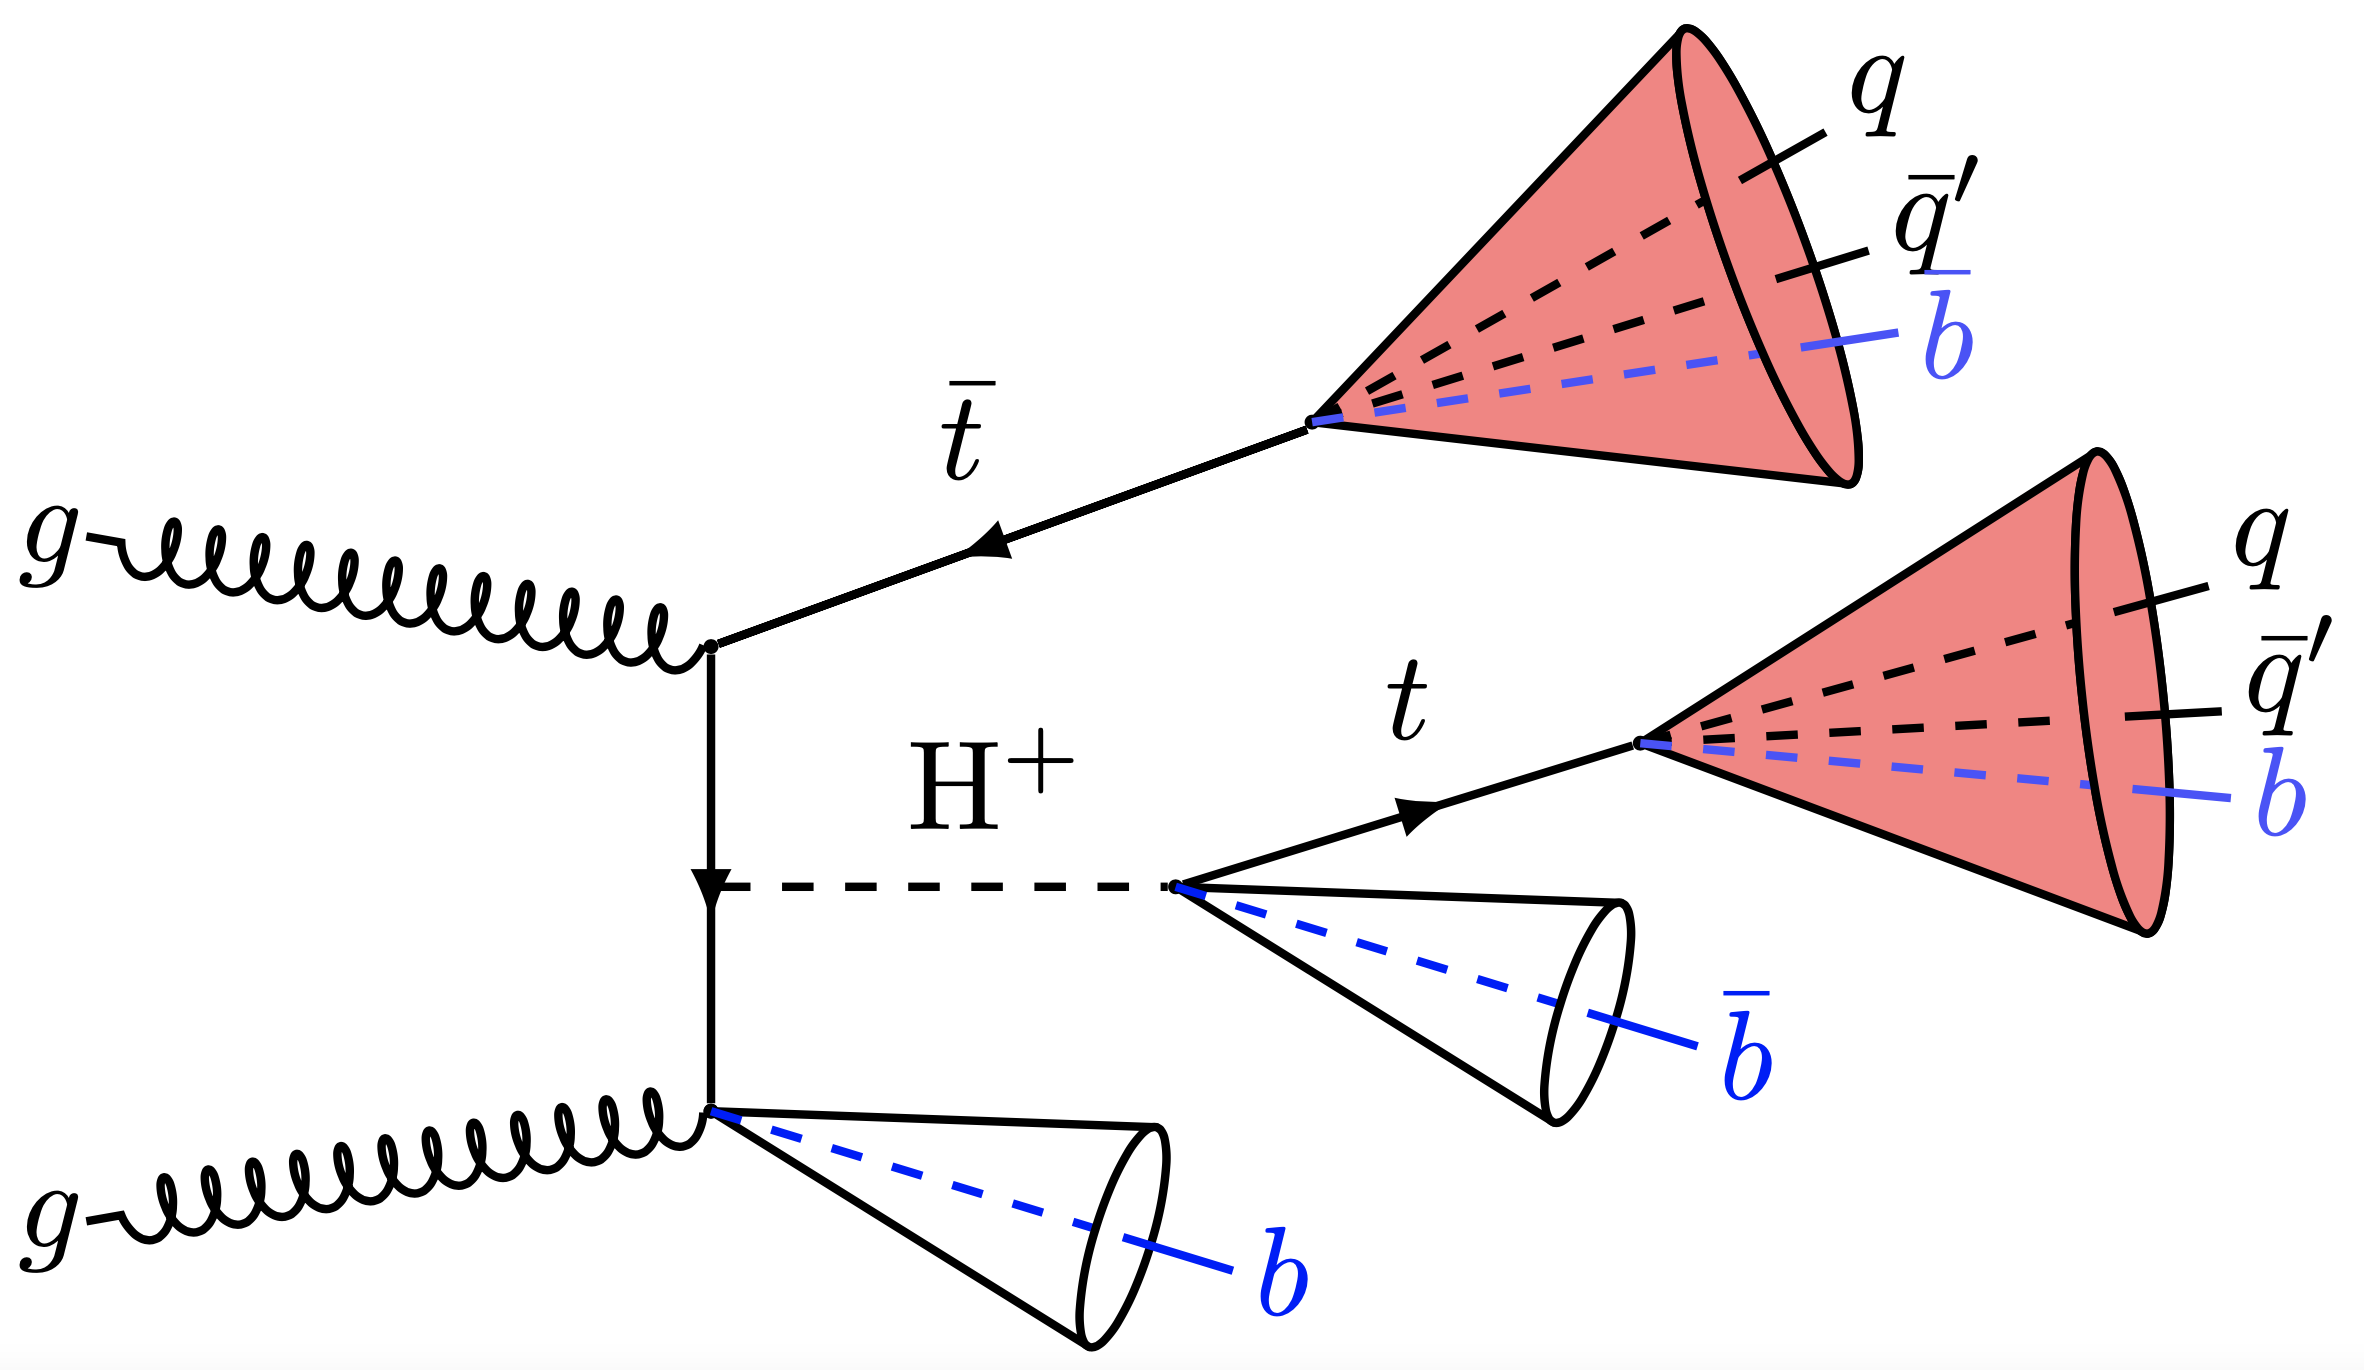
\includegraphics[width=0.2\textwidth]{./figures/boostedSR2}
        %& \\
        \hline
        \textbf{SR1} & \textbf{SR2} & \\
        \hline
        \cellcolor[gray]{.9}Trigger & \cellcolor[gray]{.9}Trigger & \cellcolor[gray]{.9}\begin{tabular}{@{}c@{}} $H_{T}$ + multijet + 1 or 2 b jets\\  $H_{T}$ + AK8 jet + trim mass $ \ \ $ \end{tabular}\\
        $\ell$ veto & $\ell$ veto & same as resolved\\
        \cellcolor[gray]{.9}$=$ 1 $t^{bst}$ &\cellcolor[gray]{.9}$=$ 2 $t^{bst}$ &  \cellcolor[gray]{.9}\pT > 400 GeV, $|\eta|$ < 2.4, \texttt{ParticleNet\_TvsQCD} Medium WP\\
        $\ge$ 4 jets & $\ge$ 2 jets & \pT > 40 GeV, $|\eta|$ < 2.4, tight ID, $H_{T}$ > 500 GeV\\
        \cellcolor[gray]{.9}$\ge$ 2 b jets & \cellcolor[gray]{.9}$\ge$ 1 b jets & \cellcolor[gray]{.9}DeepJet Medium WP \\
        $\le$ 2 $t^{res}$ & $\ge$ 0 $t^{res}$ & custom DNN loose, $130 < m_{\mathrm{t^{res}}} < 210~$GeV\\
        %\cellcolor[gray]{.9}Kinematic requirements & \cellcolor[gray]{.9}Kinematic requirements & \cellcolor[gray]{.9}\begin{tabular}{@{}c@{}}$\Delta R$($t^{bst}$, $b^{ldg}$) > 1.0\\ $\max$($m_{bb}$) > 200 GeV \end{tabular}\\         
        \cellcolor[gray]{.9}$\Delta R$($t^{bst}$, $b^{ldg}$) > 1.2 & \cellcolor[gray]{.9}$\Delta R$($t^{bst}$, $b^{ldg}$) > 0.0 & \cellcolor[gray]{.9}\\
        $\max$($m_{bb}$) > 200 GeV & $\max$($m_{bb}$) > 0 GeV & \\
        \hline
      \end{tabular}
    }
  \end{center}
  
  \twoColumnsAsymAlt
      {
        \small
        \vspace{1.0cm}
        
        $\ \ $ \textbf{Invariant \PHpm~mass reconstruction}:
        \begin{itemize}
          \normalsize
        \item[] \textcolor{kOrange}{\mHpmReco = $t^{bst}_{p_{T,1}}$ + b$^{p_{T,1}}$}
        \end{itemize}
      }
      {
        \vspace{-0.25cm}
        \oneFigColumns{tikz/pdf/HPlus4FS_HToTB_BoostedTop_InvMass}{}{0.8}%\mHpmReco=\rTop$_{ \ ldg \ p_{T}}$ + bjet$^{free}_{ldg \ p_{T}}$}{0.68}
      }
}

\MySection{Top tagging}
\Slide{t}{

  Boosted top jets $t^{bst}$ are identified using the \texttt{ParticleNet\_TvsQCD} discriminant \newline

  \vspace{-0.3cm}
  
  \small
  \textbf{Designed decorrelated tagger (DDT)}

  \vspace{0.1cm}
  \begin{itemize}
    \footnotesize
  \item \textcolor{black}{A 3D map of the \underline{tagger's score for a fixed
    mID rate} vs \pT and $\rho = \ln(m_{SD}^{2}/p_{T}^{2})$}
  \end{itemize}


  \twoFigColumns
      {DDT_particleNet_TvsQCD_0sigma.pdf}{before smearing}
      {DDT_particleNet_TvsQCD_5sigma.pdf}{5$\sigma$ Gaussian smear}
      {0.75}

      \vspace{0.1cm}
      
      \begin{itemize}
        \footnotesize
      \item Calculated with simulation QCD multijet events
      \item For each (\pT, $\rho$) bin: estimate the WP that corresponds to  $\%y$  mID rate: $X({y\%})$
      \item Transformed score: $X(DDT)$ = $X$ - $X(y\%)$ \PtRhoTag %$\rightarrow$ \textcolor{kGreen}{\pT, $\rho$ dependent}
      %\item[] $X(DDT)$ = $X$ - $X(y\%)$
      \item Selection requirment $X(DDT)$ > 0
      \end{itemize}                

%  \vspace{-0.35cm}
%  \threeFigColumnsCustomSize
%      {particleNet_TvsQCD_Rho-2.25Pt510.0.pdf}{}
%      {particleNet_TvsQCD_Rho-2.15Pt350.0.pdf}{\textcolor{black}{$X(1\%)$ in (\pT,
%        $\rho$) bins:} \vspace{0.1cm}}
%      {particleNet_TvsQCD_Rho-2.25Pt310.0.pdf}{}
%      {0.8}
}

\MySection{Background}
\Slide{t}{


  \vspace{0.1cm}
  
  %\small
  Main background:

  \begin{itemize}
    \small
  \item \ttbar (merged-t, merged-W, non-merged)
  \item QCD multijet
  \item other (minor)
  \end{itemize}
  
  \vspace{0.1cm}
  
  \begin{itemize}
    \small
  \item 2D (\mSD[t], \mHpmReco) templates derived from MC simulation
  \item Signal extraction: Signal, background simultaneous fit of (\mSD[t], \mHpmReco) 
  \end{itemize}

  \threeFigColumnsCustomSize
      {fatjet_softdropMass_BeforeDDT.png}{\mSD[t] Before TvsQCD}
      {fatjet_softdropMass.png}{\mSD[t] After TvsQCD}
      {HPlusMass_Selections.png}{\mHpmReco}
      {1.0}
}

%\MySection{Resolved}
\MySection{ }
\begin{frame}[noframenumbering]{}
  \begin{center}
    \huge \textbf{Summary}
  \end{center}
\end{frame}


\MySection{Summary}
\Slide{t}{

  \small
  Search for \PHpm $\rightarrow$ tb in fully hadronic final state presented with 2018 UL Data

  \vspace{0.2cm}

  New with respect to the previous results:

  \vspace{0.2cm}

  \begin{itemize}
    \small
  \item Three search topologies containing resolved and/or boosted tops
  \item Resolved Analysis:    
    \begin{itemize}
      \footnotesize
    \item Top tagging: custom mass-decorrelated DNN (almost published!)
    \item Event categorization based on the number of medium tagged $t^{res}$
    \item QCD background measurement shows good agreement in validation region
    \item Mass parameterized event-based tagger used as a final discriminant
    \item First expected limits with 2018 data with statistical uncertainties only
    \end{itemize}
  \item Boosted Analysis:
    \begin{itemize}
      \footnotesize
    \item boosted top indentification with \texttt{ParticleNet} (mva-based)
    \item Study new category with 1 boosted and 1 resolved top
    \item Designed decorrelated t-tagger to eliminate the mass sculpting effect
    \item Event categorization based on the number of $t^{bst}$
    \item First results show improved signal sensitivity and
      significance \FixmeTag
    \end{itemize}
  \end{itemize}
}

\MySection{Future work}
\Slide{t}{

  \vspace{0.3cm}

  
  \begin{itemize}
    \small  
  \item Resolved Analysis:    
    \begin{itemize}
      \footnotesize
    \item Incorporate the systematic uncertainties\ProgressTag
    \item Final touches on the event-based tagger\ProgressTag
    \end{itemize}
  \item Boosted Analysis:
    \begin{itemize}
      \footnotesize
    \item \texttt{ParticleNet} W/t re-calibration: Work in progress (L.Paizanos)
    \item Study the boosted W-jet category
    \item Categorization based on the top tagging rate and $N_{bjets}^{extra}$
    \item Extract SD mass templates for QCD and \ttbar (t, W, non-matched)
    \item Background data driven method \ProgressTag
    \item Produce first limits with simultaneous 2D-fit in (\mSD[t], \mHpmReco) plane
    \item Investigate using the particleNet regressed mass
    \end{itemize}
  \item Finalize and release documentation      
  \item Extend the analysis with entire Run II
  \end{itemize}

  %\vspace{1.5cm}
  %\hspace{4.8cm}
  %\large
  %\textcolor{kBlue}{\textbf{Thank you!}}
}
